\documentclass{beamer}
\usepackage{etex}
\usetheme{Antibes}
\usepackage{amssymb,amsmath,amsthm}
\usepackage{graphicx}
\usepackage{caption}
\usepackage{subfig}
\newcommand{\bn}{\begin{enumerate}[i)]}
\newcommand{\en}{\end{enumerate}}
\newcommand{\im}{\item}
\newcommand{\CPT}[1]{\large{\textbf{CHAPTER #1}}}
\newcommand{\ir}[1]{\textbf{Remark #1}}
\newcommand{\ith}[1]{\textbf{Theorem #1}}
\newcommand{\idf}[1]{\textbf{Definition #1}}
\newcommand{\iex}[1]{\textbf{Example #1}}

%\definecolor{cardinal}{rgb}{0.77, 0.12, 0.23}
%\usecolortheme[named=cardinal]{structure}
%\setbeamercolor{block title}{bg=cardinal,fg=black}
 \usepackage{tikz}
 \usetikzlibrary{patterns,snakes,plotmarks}
 \usepackage{multirow}
% \usetikzlibrary{shadows}
\usepackage{epstopdf}
\usepackage{nicefrac}
\usepackage{lmodern}
\usepackage{pgfplots}
\usepackage{qtree}
\newcommand*{\Scale}[2][4]{\scalebox{#1}{\ensuremath{#2}}}%
\DeclareCaptionLabelSeparator{horse}{:\,\,} % change according to your needs
\captionsetup{
  labelsep = horse,
  figureposition = bottom % used to get the correct vertical space between the figure and the caption
}
\setbeamertemplate{caption}[numbered]
\setbeamertemplate{items}[circle]
\setbeamertemplate{enumerate items}[square]
\theoremstyle{definition}
\newtheorem*{exs}{Examples}
\newtheorem{ex}{Example}
\newtheorem*{exc}{Exercise}
%\usepackage{booktabs}
\setlength{\parindent}{0pt}
%\setbeameroption{show notes}
 \setbeamerfont{note page}{size=\tiny}
%\setbeamertemplate{note page}[plain]
%\setbeameroption{show only notes}
\title{Math 629 - Survival Analysis \\ Chapter 5: The Stratified Cox Procedure}
\author{Drew Lazar}
\institute{Ball State University}
\date{\today}

\begin{document}
\begin{frame}
    \titlepage
\end{frame}



\section{Chapter 5}
\begin{frame}
\frametitle{The Stratified Cox Procedue}
\begin{block}{Overview}
\begin{enumerate}
\item We can deal with variables that don't satifisy the PH assumption by stratification.
\item We will see stratification by a single covariate and more than one covariate.
\item We will consider a stratified Cox PH model without and with interaction.
\end{enumerate}
\end{block}
\end{frame}

\begin{frame}
\frametitle{Stratification by covariate without interaction}
\begin{block}{Example 5.1: Remission data - stratification by Sex}
\begin{itemize}
\item We saw in chapter 4 that in the Remission data set: TR and LogWBC statisfy the PH assumption but Sex does not.
\item We can stratify on Sex (Male and Female) and create Cox PH models using TR and LogWBC in each strata. Without interaction we have:
\[
h_g(t,X) = h_{0,g}(t)\exp(\beta_1 TR + \beta_2 logWBC) \text{ for } g=1,2.
\]
\item $g$ denotes the stratum with $g=1$ for Females and $g=2$ for Males.
\item With no interaction, for both stratum the effect of a unit increase of a covariate on the hazard (HR) is the same.
\end{itemize}
\end{block}
\end{frame}

\begin{frame}
\frametitle{Stratification by covariate without interaction (cont'd)}
\begin{block}{Problem 5.1: Remission data - stratification by Sex}
\begin{enumerate}
\item In R, fit a stratified Cox PH model to the Remission Data. Use TR and LogWBC as covariates and stratify on Sex.
\item Use a Wald test to test for the significance of TR and LogWBC.
\item Use a Likelihood ratio test to 1) test for the significance of TR and logWBC and 2) test for the significance of TR with LogWBC in the model.
\item Interpret the coefficients of TR and LogWBC in the stratified Cox PH model.
\item Plot adjusted survival curves for TR from your Stratified Cox PH model. Set logWBC=mean(logWBC).
\end{enumerate}
\end{block}
\end{frame}

\begin{frame}
\frametitle{Stratification by covariate without interaction (cont'd)}
\begin{block}{The General Statified Cox (SC) Model}
\begin{enumerate}
\item We describe the general form of the SC model that allows for stratification of several predictors.
\item We have $k$ variables not satisfying the PH assumption and $p$ variables satisfying the PH assumption.
\item $Z_1, Z_2,. . ., Z_k$ do not satisfy PH. $X_1, X_2,. . ., X_p$ satisfy PH.
\item We proceed as follows:
\begin{enumerate}
\item Categorize each $Z_i$.
\item Form $k^*$ combinations of categories.
\item The strata are the categories of $Z^*$.
\end{enumerate}
\end{enumerate}
\end{block}
\end{frame}

\begin{frame}
\frametitle{Stratification by covariate without interaction (cont'd)}
\begin{block}{The General Statified Cox (SC) Model (cont'd)}
Example with age and treatment. Age is interval variable so we stratify it.
   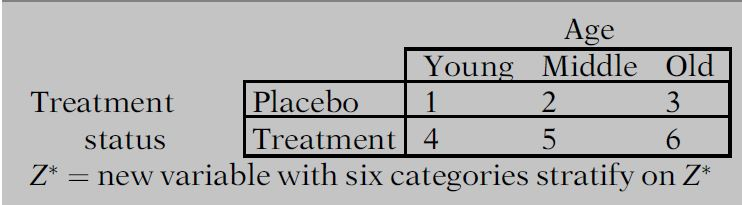
\includegraphics[width =\textwidth, height=4cm]{CH5_exampleSC}
\end{block}
\end{frame}

\begin{frame}
\frametitle{Stratification by covariate without interaction (cont'd)}
\begin{block}{The General Statified Cox (SC) Model (cont'd)}
\begin{enumerate}
\item The general SC model:
\[
h_g(t,X) = h_{0g}(t)exp(\beta_1 X_1 + \ldots + \beta_p X_p) \text{ for }  g=1,\ldots,k*
\]
\item Different baseline hazard functions: $h_{0,g}(t), g=1,\ldots,k^*$ but same coefficients $\beta_1, \ldots, \beta_p$.
\item Without interaction, the effect of a unit increase of a covariate, $X_i$, on the hazard (i.e., the HR) is $\exp(\beta_i)$.
\end{enumerate}
\end{block}
\end{frame}

\begin{frame}
\frametitle{Stratification by covariate without interaction (cont'd)}
\begin{block}{The General Statified Cox (SC) Model (cont'd): Maximum Likelihood Estimation}
\begin{itemize}
\item We obtain estimates for $\beta_1,\ldots,\beta_p$ by partial maximum likelihood estimation.
\item We maximize a partial likelihood function, $L$, that is obtained by multiplying together likelihood functions for each
stratum as shown below.
\vspace{10pt}
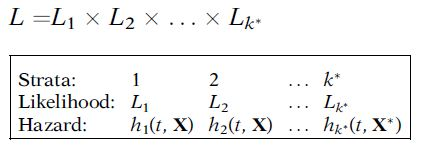
\includegraphics[width =\textwidth, height=3.2cm]{CH5_Partiallike}
\end{itemize}
\end{block}
\end{frame}


\begin{frame}
\frametitle{Stratification by covariate with interaction}
\begin{block}{Example 5.2: Remission data - stratification by Sex with interaction}
\begin{itemize}
\item Without interaction our SC model is
\[
h_g(t,X) = h_{0,g}(t)\exp(\beta_1 TR + \beta_2 logWBC) \text{ for } g=1,2.
\]
\item With interaction our SC model is
\begin{equation} \label{eq:Int1}
h_g(t,X) = h_{0,g}(t)\exp(\beta_{1g} TR + \beta_{2g} logWBC) \text{ for } g=1,2.
\end{equation}
\item With interaction the HR's depend on the strata. For example, for females ($g=1$) the effect of a unit increase in TR on the hazard is
\[
\exp(\beta_{1g}) \text{ for } g=1,2.
\]
\end{itemize}
\end{block}
\end{frame}

\begin{frame}
\frametitle{Stratification by covariate with interaction (cont'd)}
\begin{block}{Example 5.2: Remission data - stratification by Sex with interaction (cont'd)}
\begin{itemize}
\item An alternative interaction model is a follows:
\begin{equation}\label{eq:Int2}
\begin{aligned}
h_g(t,X) & = h_{0,g}(t)\exp[\beta_1^*\ TR + \beta_2^*\ logWBC +  \\
& \beta_3^*(Sex*TR) + \beta_4^*(Sex*logWBC) ] \text{ for } g=1,2.
\end{aligned}
\end{equation}
\item Stratified interaction models \eqref{eq:Int1} and \eqref{eq:Int2} are, in fact, equivalent models.
\end{itemize}
\end{block}
\end{frame}

\begin{frame}
\frametitle{Stratification by covariate with interaction (cont'd)}
\begin{block}{Example 5.2: Remission data - stratification by Sex with interaction (cont'd)}
How are \eqref{eq:Int1} and \eqref{eq:Int2} equivalent?
\begin{itemize}
\item Using model \eqref{eq:Int1}, the effect of a unit increase in TR, i.e., HR(TR), is:
\[ \beta_{11} \text{ for } g=1 \text{ and }  \beta_{12} \text{ for } g=2.
\]
\item Using model \eqref{eq:Int2}, the effect of a unit increase in TR, i.e., HR(TR), is:
\[
\beta_{1}^* + \beta_{3}^**\text{Sex}.
\]
\item Thus, $\beta_{11}=\beta_{1}^*$ and  $\beta_{12}=\beta_{1}^*+\beta_{3}^*$.
\item Similarily, we have $\beta_{21}=\beta_{2}^*$ and  $\beta_{22}=\beta_{2}^*+\beta_{4}^*$.
\end{itemize}
\end{block}
\end{frame}

\begin{frame} 
\frametitle{Stratification by covariate with interaction (cont'd)}
\begin{block}{Problem 5.2: Remission data - stratification by Sex with interaction}
\begin{enumerate}
\item In R, fit a stratified Cox PH model to the Remission Data. Use TR and LogWBC as covariates and stratify on Sex. Assume interaction of the covariates with sex.
\item In R, test the interaction assumption using a likelihood ratio test.  
\item Using the interaction model, find HR of TR for Sex=0 (female) and Sex=1 (male). 
\end{enumerate} 
\end{block} 
\end{frame} 
\end{document}

